% siminos/spatiotemp/Examples/examC3cosets.tex
% $Author: predrag $ $Date: 2021-08-30 01:52:26 -0400 (Mon, 30 Aug 2021) $

%%%%%%%%%%%%%%%%%%%%%%%%%%%%%%%%%%%%%%%%%%%%%%%%%%%
\begin{figure}
  \centering
  \begin{minipage}[b]{0.98\textwidth}
(a)~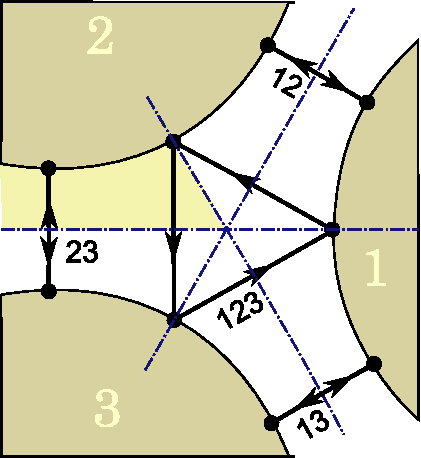
\includegraphics[width=0.25\textwidth]{3diskSymm-0}%
~~(b)~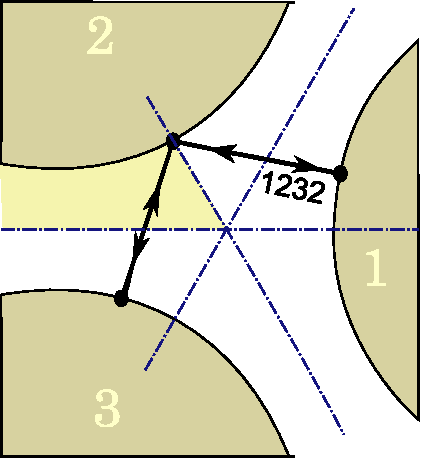
\includegraphics[width=0.25\textwidth]{3diskSymm-01}%
~~(c)~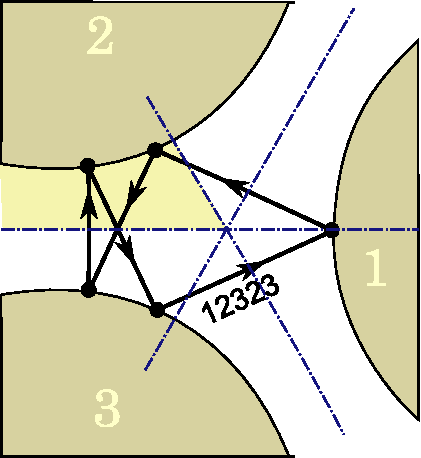
\includegraphics[width=0.25\textwidth]{3diskSymm-00111}
\vskip 2ex %\\
(d)~~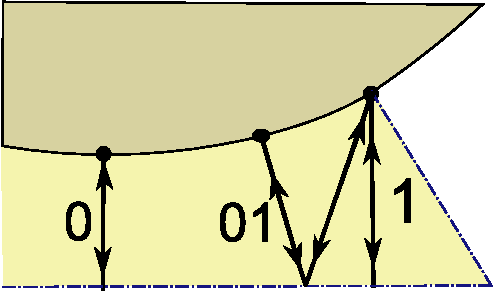
\includegraphics[width=0.25\textwidth]{3diskFundD}
  \end{minipage}
  \caption{\label{fig:3diskSymm}
% Following overhead on ChaosBook.org/overheads:
% \\
The 3-disk pinball {\orbit}s:
(a)
\cycle{12}, \cycle{13}, \cycle{23}, \cycle{123};
the clockwise \cycle{132} not drawn.
(b)
{\Orbit} \cycle{1232}; the symmetry related
\cycle{1213} and \cycle{1323} not drawn.
(c)
{\Orbit} \cycle{12323}; {\orbit}s \cycle{12123}, \cycle{12132}, \cycle{12313},
\cycle{13131} and \cycle{13232} not drawn.
(d) The fundamental domain, \ie, the light-shaded 1/6th wedge in
(a), consisting of a section of a disk, two segments of
symmetry axes acting as straight mirror walls, and the escape
gap to the left. The above 14 full-space {\orbit}s restricted to
the fundamental domain and recoded in binary reduce to the two
fixed points \cycle{0}, \cycle{1}, period-2 {\orbit} \cycle{10}, and
period-5 {\orbit} \cycle{00111} (not drawn).
% Radius~:~center separation ratio a:R~=~1:2.5.
}
\end{figure}
%%%%%%%%%%%%%%%%%%%%%%%%%%%%%%%%%%%%%%%%%%%%%%%%%%%

%%%%%%%%%%%%%%%%%%%%%%%%%%%%%%%%%%%%%%%%%%%%%%%%%%%%%%%%%%%%%%%%%%
\example{Subgroups, cosets of \Dn{3}.}{ \label{exam:C3cosets}
% examFiniteGr.tex called by \Chapter{finiteGr}{}{Flips, slides and turns}
\index{three-disk@3-disk!symmetry}\index{symmetry!3-disk}          \toCB
~~~(Continued from \refexam{exam:C3vInv})\\
The 3-disks symmetry group, the \Dn{3} dihedral group \refeq{groupD3}
has six subgroups
\beq
\{e\},\quad
\{e, \Refl\},\;
\{e, \Refl_{1}\},\;
\{e, \Refl_{2}\},\quad
\{e, \shift, \shift_2\},\quad
\Dn{3}
\,.
\ee{D3subgr}
The left cosets of subgroup $\Dn{1} = \{e, \Refl\}$ are
$\{\shift,\Refl_{1}\}$,
$\{\shift_2,\Refl_{2}\}$.
The coset of subgroup $\Cn{3} = \{e, \shift, \shift_2\}$ is
$\{\Refl,\Refl_{1},\Refl_{2}\}$. The significance of the
coset is that if a solution has a symmetry $H$, for example the symmetry
of a 3-cycle $\overline{123}$ is $\Cn{3}$, then all elements in a coset
act on it the same way, for example
$\{\Refl,\Refl_{1},\Refl_{2}\} \overline{123} = \overline{132}$.

The nontrivial subgroups of $\Dn{3}$ are $\Dn{1} = \{ e, \sigma \}$, consisting
of the identity and any one of the reflections, of order 2, and $\Cn{3} =
\{ e, \shift, \shift_2 \}$, of order $3$, so possible cycle
multiplicities are $|\Group|/|\Group_{p}| = 1$, $2$, $3$ or $6$. Only the
fixed point at the origin has full symmetry $\stab{p}=\Group$. Such
\eqva\ exist for smooth potentials, but not for the 3-disk billiard.
Examples of other multiplicities are given in \reffig{fig:3diskSymm} and
\reffig{dscr:fg3-exam}.
~~(continued in \refexam{exam:3diskClass})
                                        \jumpBack{exam:C3cosets}
    } %end \example{$D_3$ invariance - 3-disk game of pinball
%%%%%%%%%%%%%%%%%%%%%%%%%%%%%%%%%%%%%%%%%%%%%%%%%%%%%%%%%%%%%%%%%%
